\documentclass[12pt,letterpaper, onecolumn]{exam}
\usepackage{amsmath}
\usepackage{amssymb}
\usepackage{amsthm}
\usepackage{graphicx}
\usepackage{mathrsfs}
\usepackage{xcolor}
\usepackage[lmargin=71pt, tmargin=1.2in]{geometry}  %For centering solution box
\usepackage[english]{babel}
\newtheorem{theorem}{Theorem}
\newtheorem{lemma}[theorem]{Lemma}
\usepackage{accents}
\usepackage{ulem} % sout() to cros\sing things out 
\newcommand{\ubar}[1]{\underaccent{\bar}{#1}}
\newcommand{\bs}[1]{\boldsymbol{#1}}
\newcommand{\bm}[1]{\mathbf{#1}}
\newcommand{\der}[2]{\frac{d #1}{d#2}}
\newcommand{\pder}[3]{\frac{\delta^{#3} #1}{\delta^{#3}#2}}
\newcommand{\rs}{$X_1, ..., X_n$}
\newcommand{\nsum}{\sum_{i=1}^n}
\newcommand{\nprod}{\prod_{i=1}^n}
\newcommand*{\Comb}[2]{{}^{#1}C_{#2}}%
\newcommand{\ifc}{\textrm{ if }}
\newcommand{\real}{\mathbb{R}}
\newcommand{\nat}{\mathbb{N}}
\newcommand{\power}{\mathcal{P}}
\newcommand{\rational}{\mathbb{Q}}
\newcommand{\cutelim}{\lim\limits_{n\to\infty}}
\newcommand{\salg}{$\sigma$-algebra }

\newcommand{\calA}{\mathcal{A}}
\newcommand{\calO}{\mathcal{O}}
\newcommand{\calC}{\mathcal{C}}
\newcommand{\calB}{\mathcal{B}}
\newcommand{\calI}{\mathcal{I}}
\newcommand{\calF}{\mathcal{F}}
\newcommand{\calG}{\mathcal{G}}
\newcommand{\I}{\mathbf{I}}
\newcommand{\gensig}[1]{\sigma\langle #1 \rangle} % notation for a sigma algebra generated by some set 
\newcommand{\om}{\mu^*} % outer measure 
\newcommand{\rat}{\mathbb{Q}}
\newcommand{\tribrac}[1]{\langle #1 \rangle}
\newcommand{\Borel}{\mathcal{B}(\mathbb{R})}
\newcommand{\Boreltwo}{\mathcal{B}(\mathbb{R}^2)}
\newcommand{\Borelk}[1]{\mathcal{B}(\mathbb{R}^#1)}
\newcommand{\probspace}{(\Omega, \calF, P)}

\newcommand{\Iunion}{\bigcup_{\alpha \in I}}
\newcommand{\Iintersect}{\bigcap_{\alpha \in I}}

\newcommand{\dm}{d \mu}

\newcommand{\cutesum}[1]{\sum_{#1 = 1}^\infty}


% \chead{\hline} % Un-comment to draw line below header
\thispagestyle{empty}   %For removing header/footer from page 1

\begin{document}

\begingroup  
    \centering
    \LARGE STAT 6410\\
    \LARGE Homework \\[0.5em]
    \large Sarah Kilgard\par
\endgroup
\rule{\textwidth}{0.4pt}
\pointsdroppedatright   %Self-explanatory
\printanswers
\renewcommand{\solutiontitle}{\noindent\textbf{Ans:}\enspace}   %Replace "Ans:" with starting keyword in solution box

\begin{questions}
%%%%%%%%%%% Question 1 %%%%%%%%%%%%%%%%%%%%    
    \question Chapter 5, Problem 1 \\
    Verify that if $\mu_1$ and $\mu_2$ are finite measures on $(\Omega_1, \calF_1)$ and $(\Omega_2, \calF_2)$, respectively, then $\mu_{12}(\cdot)$ and $\mu_{21}(\cdot)$, defined by (1.4) and (1.5), respectively, are measures on $(\Omega_1  \times  \Omega_2, \calF_1  \otimes \calF_2)$. \\ (\textbf{Hint}: Use the MCT.) \\
    \underline{Note:}
    \[\mu_{12}(A) = \int_{\Omega_1} \mu_2(A_{1\omega_1})\mu_1 d(\omega_1) \quad \mu_{21}(A) = \int_{\Omega_2} \mu_1(A_{2\omega_2})\mu_2 d(\omega_2)\]
    \begin{solution}
        \textbf{WTS} $\mu_{12}(\cdot)$ is a measure on $(\Omega_1  \times  \Omega_2, \calF_1  \times \calF_2)$.
        \begin{itemize}
            \item $\mu_2(\emptyset) = \int_{\Omega_1} \mu_2(\emptyset_{1 \omega_1} \mu_1 d(\omega_1) = \int_{\Omega_1} \mu_2(\emptyset) d\mu_1(\omega_1) = 0$
            \item Since $\mu_2(A_{1\omega_1})$ is a nonnegative measurable function, the integral of it will also be nonnegative
            \item Define $D \in \calF_1 \otimes \calF_2$. Define $\{A_n\}_{n \geq 1}$ to be a disjoint sequence of sets in $\calF_1 \otimes \calF_2$ such that $D = \cup_{n\geq1}A_n$
            \begin{align*}
                & \mu_{12}(D) = \int_{\Omega_1}\mu_2(D_{1\omega_1})\mu_1d(\omega_1) \\
                & \textrm{From Prop 5.1.1, we know for each } \omega_1 \in \Omega_1, A_{n 1 \omega_1} \in \calF_2 \\
                & \therefore \: \mu_{12}(D) = \int_{\Omega_1}\mu_2(\cup_{n\geq 1} A_{n 1 \omega_1})\mu_1d(\omega_1) \\ 
                & \mu_2 \textrm{ is a measure and, } \{A_{n 1 \omega_1}\}_{n \geq 1} \textrm{ is disjoint, } \\
                & \mu_{12}(D) = \int_{\Omega_1}\sum_{n\geq 1}\mu_2( A_{n 1 \omega_1})\mu_1d(\omega_1) \\
                & \textrm{For each n, } \mu_2(A_{n 1 \omega_1} \textrm{ is a nonnegative measurable function, so by MCT:} \\
                & \mu_{12}(D) = \int_{\Omega_1}\mu_2(\cup_{n\geq 1} A_{n 1 \omega_1})\mu_1d(\omega_1) = \sum_{n\geq 1} \int_{\Omega_1}\mu_2( A_{n 1 \omega_1})\mu_1d(\omega_1)
            \end{align*}
        \end{itemize}
        Thus, $\mu_{12}(\cdot)$ is a measure on $(\Omega_1 \times \Omega_2, \calF_1 \otimes \calF_2)$

        In the same way, we can also show that $\mu_{21}(\cdot)$ is a measure on $(\Omega_1 \times \Omega_2, \calF_1 \otimes \calF_2)$
    \end{solution}

%%%%%%%%%%% Question 2 %%%%%%%%%%%%%%%%%%%%    
    \question Chapter 5, Problem 6\\
    Let $(\Omega, \calF,\mu)$ be a $\sigma$-finite measure space and $f$ be a nonnegative measurable function. Then, 
    $\int_\Omega fd\mu = \int_{[0,\infty)}\mu(\{f \geq t\})dt. $ \\ (\textbf{Hint:} Consider the product space of $(\Omega, \calF,\mu)$ with $(\real_+, \calB(\real_+),m)$ and apply Tonelli’s theorem to the function $g(\omega, t)=I(f(\omega) \geq t)$, after showing that $g$ is $\calF \otimes \calB(\real_+)$-measurable.)

    \begin{solution}
        \begin{proof}
            \textbf{WTS:} $g$ is $\calF \otimes \calB(\real_+)$-measurable

            $g(\omega, t) = I(f(\omega) \geq t) = I_{\{(\omega, t) \in \Omega \times \real_+: f(\omega) \geq t\}}(\omega, t)$

            $f(\omega)$ is $\calF$ measurable and $t$ is $\calB(\real_+)$ measurable, so $\{(\omega, t) \in \Omega \times \real_+: f(\omega) \geq t\} \in \calF \otimes \calB(\real_+)$.

            Thus, $g(\omega, t)$ is $\calF \otimes \calB(\real_+)$- measurable, since it is an indicator function for a $\calF \otimes \calB(\real_+)$-measurable set.

            Clearly, $g(\omega, t)$ is a nonnegative function as it can only take on the values 0 and 1. Thus, we can use Tonelli's theorem.
            
            \begin{align*}
                & k_1(\omega) = \int_{\real_+}g(\omega, t) m (d t) = \int_{\real_+} I(f(\omega) \geq t) m(dt) = m(\{(\omega, t) \in \Omega \times \real_+: f(\omega) \geq t\}) = f \\
                & k_2(t) = \int_{\Omega}g(\omega, t) \mu (d \omega) = \int_{\Omega}I(f(\omega) \geq t)) \mu (d \omega) = \mu(\{f \geq t\}) \\
                & \textrm{From Tonelli's Theorem, we know that } \int_{\Omega}k_1 d\mu = \int_{\real_+}k_2 dm = \int_{[0, \infty)]k_2(t) dt} \\
                & \therefore \; \int_{\Omega}fd\mu = \int_{[0, \infty)]}\mu(f(\omega) \geq t) dt
            \end{align*}
        \end{proof}
    \end{solution}

%%%%%%%%%%% Question 3 %%%%%%%%%%%%%%%%%%%%    
    \question Chapter 5, Problem 10 \\
    Show that $I \equiv \int_0^\infty e^{-x^2/2}dx = \sqrt{\frac{\pi}{2}}$
    (\textbf{Hint}: By Tonelli’s theorem, $I^2 = \int_0^\infty e^{-\frac{(x^2 + y^2)}{2}}dxdy$. Now use the change of variables $x = r \cos \theta$, $y = r \sin \theta$, $0<r<\infty$, $0<\theta< \frac{\pi}{2}$.)

    \begin{solution}
        \begin{align*}
            & I = \int_0^\infty e^{-x^2/2}dx = \int_0^\infty e^{-y^2/2}dy \\
            & \textrm{By Tonelli's theorem:} I^2 = \int_0^\infty e^{-\frac{(x^2 + y^2)}{2}}dxdy \\
            & \textrm{Now we will use the change of variables where:} x = r \cos(\theta) \: \& \: y = r \sin(\theta) \\
            & I^2 = \int_0^\infty \int_0^{\tfrac{\pi}{2}} e^{-((r\cos(\theta))^2 + (r\sin(\theta))^2)/2}J d\theta dr, \: \textrm{where J is the Jacobian} \\
            & J = \frac{d}{dr}r\cos(\theta) \frac{d}{d\theta}r\sin(\theta) -\frac{d}{d\theta}r\cos(\theta) \frac{d}{dr}r\sin(\theta) = r \\
            & I^2 = \int_0^\infty \int_0^{\tfrac{\pi}{2}} e^{-(r^2(\cos(\theta)^2 + \sin(\theta)^2)/2}r d\theta dr = \int_0^\infty\int_0^{\tfrac{\pi}{2}} e^{-r^2/2}r d\theta dr \\
            & = \int_0^\infty \left[e^{-r^2/2}r\left(\frac{\pi}{2}\right) - e^{-r^2/2}r(0)\right]dr \\
            & = \frac{\pi}{2}\int_0^\infty re^{-r^2/2}dr \\
            & \frac{d}{dr}\left(-e^{-r^2/2}\right) = re^{-r^2/2} \\
            & I^2 = \frac{\pi}{2}\int^\infty_0 \frac{d}{dr}\left(-e^{-r^2/2}\right)dr = \frac{\pi}{2}\left[-e^{-r^2/2}\right]_0^\infty = \frac{\pi}{2}(0 - - 1) = \frac{\pi}{2} \\
            & \therefore \: I = \sqrt{I^2} = \sqrt{\frac{\pi}{2}}
        \end{align*}
    \end{solution}
    
\clearpage

%%%%%%%%%%% Question 4 %%%%%%%%%%%%%%%%%%%%    
    \question Chapter 5, Problem 11 \\
    Let $\mu$ be a finite measure on $(\real, \Borel)$. Let $f, g: \real \to \real_+$ nondecreasing. Show that
    \[\mu(\real)\int fg d\mu \geq \left(\int f d\mu\right) \left(\int g d \mu\right)\]
    (\textbf{Hint}: Consider $h(x_1,x_2)=(f(x_1) - f(x_2))(g(x_1) - g(x_2))$ on  $\real^2 $ and integrate w.r.t. $\mu  \times  \mu$.)
    
    \begin{figure}[h!]
        \centering
        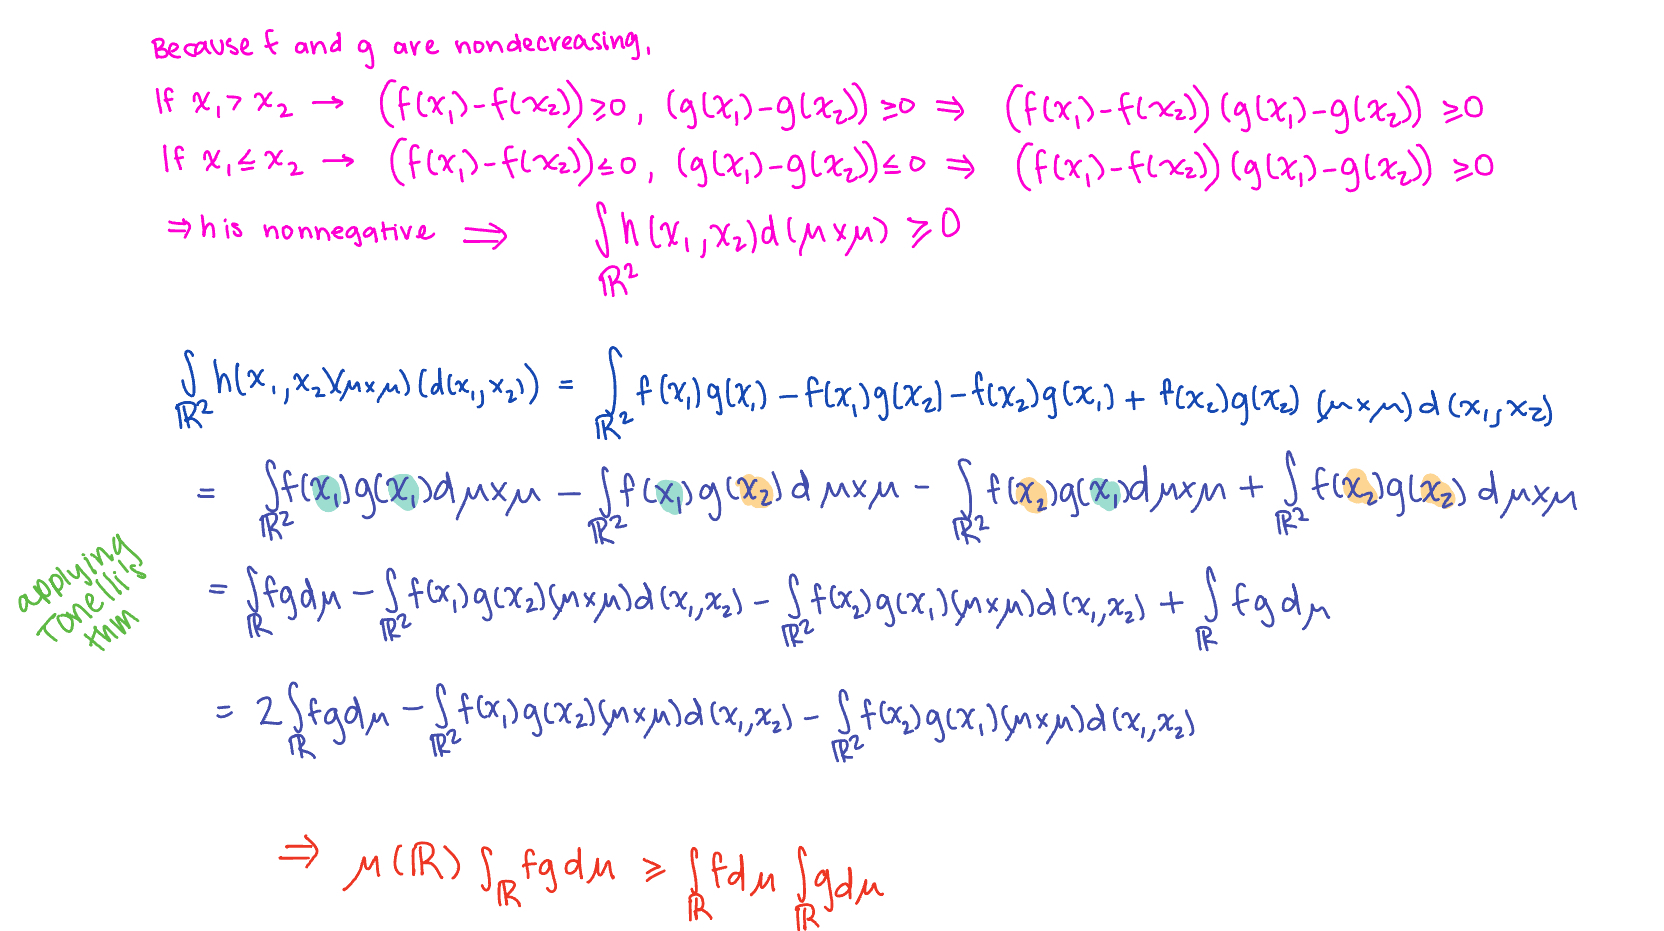
\includegraphics[width=1.25\linewidth]{hw9.png}
    \end{figure}

    \clearpage

%%%%%%%%%%% Question 4 %%%%%%%%%%%%%%%%%%%%    
    \question Problem A

    Consider the following measure spaces \\
    $(\Omega_i = \nat, \calF_i = \power(\nat)$, $\mu_i$ = counting measure), $i = 1, 2$. \\
    Define $f : (\Omega_1 \times \Omega_2) \rightarrow \real$ as
    \[f(\omega_1, \omega_2) = \I_{\{(n, n): \: n\in \nat\}}(\omega_1, \omega_2) - \I_{\{(n, n + 1) : \: n\in \nat\}}(\omega_1, \omega_2)\]
    Then,
    \begin{itemize}
    \item[(i)] Prove $\calF_1 \otimes \calF_2 = \power (\nat \times \nat)$.
    \item[(ii)] Is $f$ a $\calF_1 \otimes \calF_2$ measurable function?
    \item[(iii)] Is $f$ integrable w.r.t $\mu_1 \times \mu_2$?
    \item[(iv)] Compute the two iterated integrals:
    \[\int_{\Omega_1} \left[\int_{\Omega_2} f(\omega_1, \omega_2) d \mu_2(\omega_2)\right]d\mu_1(\omega_1), \quad \int_{\Omega_2}\left[\int_{\Omega_1} f(\omega_1, \omega_2) d\mu_1(\omega_1)\right]d\mu_2(\omega_2)\]
    
    \end{itemize}

    \begin{solution}
    (i) \begin{proof}
        \textbf{WTS:} $\power(\nat) \otimes \power(\nat) \subseteq \power(\nat \times \nat) $ \\
       Both are \salg on $\nat \times \nat$, and $\power(\nat \times \nat)$ is the largest \salg on $\nat \times \nat$. Thus: $\power(\nat) \otimes \power(\nat) \subseteq \power(\nat \times \nat) $ 
       
        \textbf{WTS:} $\power(\nat \times \nat) \subseteq \power(\nat) \otimes \power(\nat)$ \\
        $\power(\nat) \otimes \power(\nat) = \gensig{\{ A_1 \times A_2: A_1, A_2 \in \power(\nat)\}}$

        Suppose $A \in \power(\nat \times \nat)$. Thus, there exist $a_1, a_2, ... \in \nat$ and $b_1, b_2, ... \in \nat$ such that $A = \cup_{n \geq 1} \{(a_n, b_n)\}$ (since $\nat \times \nat$ is countable). 

        Clearly, $\{(a_n, b_n)\} \in \power(\nat) \otimes \power(\nat)$ for all $n \geq 1$. Thus, $A \in \power(\nat) \otimes \power(\nat)$ since a \salg is closed under countable unions.

        Thus, $\power(\nat \times \nat) \subseteq \power(\nat) \otimes \power(\nat)$.

        So $\power(\nat \times \nat) = \power(\nat) \otimes \power(\nat) = \calF_1 \otimes \calF_2$
        \end{proof}
        (ii) Yes, $f$ is a simple function and the sets associated with each indicator, $\{(n, n): n \in \nat\}$ and $\{(n, n + 1): n \in \nat\}$ are both elements of $\calF_1 \otimes \calF_2$.

        (iii) 
        \begin{align*}
            & \int_{\nat \times \nat} |f| d \mu_1 \times \mu_2  \\
            & = \int_{\nat \times \nat}  \I_{\{(n, n): \: n\in \nat\}}(\omega_1, \omega_2) + \I_{\{(n, n + 1) : \: n\in \nat\}}(\omega_1, \omega_2) d \mu_1 \times \mu_2 (\omega_1, \omega_2) \\
            & = 1 \cdot \mu_1\times \mu_2(\{(n, n): \: n\in \nat\}) + 1 \cdot \mu_1\times \mu_2(\{(n, n+1): \: n\in \nat\}) \\
            & = 1 \cdot \infty + 1 \cdot \infty = \infty 
        \end{align*}
        Thus, f is not integrable w.r.t $\calF_1 \otimes \calF_2$.

        (iv) 
        \begin{align*}
            & \int_{\Omega_1} \left[\int_{\Omega_2} f(\omega_1, \omega_2) d \mu_2(\omega_2)\right]d\mu_1(\omega_1) \\
            & = \int_{\Omega_1} \left[\int_{\Omega_2} \I_{\{(n, n): \: n\in \nat\}}(\omega_1, \omega_2) - \I_{\{(n, n + 1) : \: n\in \nat\}}(\omega_1, \omega_2) d \mu_2(\omega_2)\right]d\mu_1(\omega_1) \\
            & = \int_{\Omega_1}\left[\mu_2(\{(\omega_1, n): \: n = \omega_1\}) - \mu_2(\{(\omega_1, n + 1): \: n = \omega_1 + 1\})\right]d \mu_1(\omega_1) \\
            & = \int_{\Omega_1} 0 d \mu_1(\omega_1) = 0
        \end{align*}

        \begin{align*}
            & \int_{\Omega_2} \left[\int_{\Omega_1} f(\omega_1, \omega_2) d \mu_1(\omega_1)\right]d\mu_2(\omega_2) \\
            & = \int_{\Omega_2} \left[\int_{\Omega_1} \I_{\{(n, n): \: n\in \nat\}}(\omega_1, \omega_2) - \I_{\{(n, n + 1) : \: n\in \nat\}}(\omega_1, \omega_2) d \mu_1(\omega_1)\right]d\mu_2(\omega_2) \\
            & = \int_{\Omega_2}\left[\mu_1(\{(n, \omega_2): \: n = \omega_2\}) - \mu_1(\{(n, \omega_2): \: n = \omega_2 - 1 \})\right]d \mu_2(\omega_2) \\
            & = \int_{\Omega_1} 0 d \mu_2(\omega_2) = 0
        \end{align*}

        
    \end{solution}


\end{questions}
\end{document}